\section{Procedure}
\label{sec:procedure}

\subsection{Synthesis}
\label{sec:synthesis}

\subsection{4-probe measurement}
\label{sec:4-probe measurement}
Since normal voltmeters have a high error due to contact resistance. Therefore, we measure the
resitance using 4 probes which circumvent this issue
\cite{Hofmann_2009,https://doi.org/10.1002/j.1538-7305.1958.tb03883.x}. A sketch of a sample with
four probes attached and the wiring is shown in \autoref{fig:4-probe-setup}. For this type of
measurement, four probes have to be attached to the sample in a row. A voltage source creates a
voltage between the outer probes (probe 1 and 4 in \autoref{fig:4-probe-setup}) and the current $A$ is
measured. Between the inner probes (2 and 3 in \autoref{fig:4-probe-setup}) the voltage $V$ is measured.
The resistance can be calculated using Ohm`s law
\begin{equation}
  R = \frac{A}{V}.
\end{equation}
Although when considering the resistance of the whole sample another factor appears which relates to
shape and dimensions of the sample.

To minimize the resistance created by the probes, the surface area when contacting the sample has to be
maximized. This has been accomplished by wrapping each probe once around the sample using
soldering alloys. Special attention has to be given to the solder of different probes not touching each
other.

\begin{figure}
  \centering
  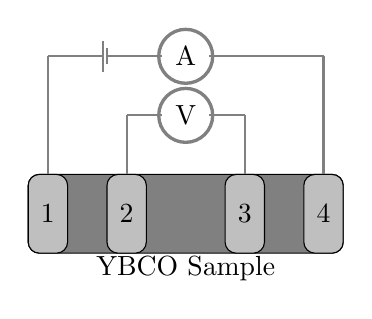
\begin{tikzpicture}
    [roundnode/.style={circle, draw=gray, very thick, minimum size=4mm}]
    \draw[rounded corners,fill=gray] (0, 0) rectangle (4, 1) {};

    \draw[rounded corners,fill=lightgray] (0, 0) rectangle (0.5, 1) {};
    \draw[rounded corners,fill=lightgray] (1, 0) rectangle (1.5, 1) {};
    \draw[rounded corners,fill=lightgray] (2.5, 0) rectangle (3, 1) {};
    \draw[rounded corners,fill=lightgray] (3.5, 0) rectangle (4, 1) {};

    \draw[gray, thick] (0.25,1) -- (0.25,2.5);
    \draw[gray, thick] (3.75,1) -- (3.75,2.5);

    \draw[gray, thick] (2.3,2.5) -- (3.75,2.5);
    \draw[gray, thick] (1,2.5) -- (1.7,2.5);
    \node[roundnode] at (2,2.5) {A};
    \draw[gray, thick] (1,2.4) -- (1,2.6);
    \draw[gray, thick] (0.95,2.3) -- (0.95,2.7);
    \draw[gray, thick] (0.95,2.5) -- (0.25,2.5);

    \draw[gray, thick] (1.25,1) -- (1.25,1.75);
    \draw[gray, thick] (2.75,1) -- (2.75,1.75);

    \draw[gray, thick]  (1.25,1.75) -- (1.7,1.75);
    \draw[gray, thick]  (2.3,1.75) -- (2.75,1.75);
    \node[roundnode] at (2,1.75) {V};

    \node[] at (2,-0.2) {YBCO Sample};

    \node[] at (0.25,0.5) {1};
    \node[] at (1.25,0.5) {2};
    \node[] at (2.75,0.5) {3};
    \node[] at (3.75,0.5) {4};
  \end{tikzpicture}
    \caption{4-probe setup to measure the electrical resistance of a YBCO crystal. While a voltage
      is created and current measured between probe 1 and 4, the voltage is measured between the
    inner probes 2 and 3.}
  \label{fig:4-probe-setup}
\end{figure}


